\chapter{Methodology}
\label{chapter:methodology-overview}

This chapter presents the methodological framework of the thesis. Building on the problem definition in Chapter~\ref{chapter:objectives-problem}, it describes the event-driven simulation environment, the way relocation guidance from the upstream OR model enters the execution layer, and the formulation of the trip-level refinement problem for reinforcement-learning-based evaluation. The emphasis is on the operational logic of the framework rather than on the internal formulation of the upstream rebalancing model.

\section{Methodological Overview}

% \subsection{Layered Framework}

% The methodology follows a layered structure. The upstream layer is an OR model or rebalancing model that produces interval-based relocation guidance. In this thesis, these outputs are treated as external inputs. The downstream layer is a trip-level refinement mechanism that decides whether a relocation suggestion should actually be activated when an eligible trip request is realized. The simulation environment connects these two layers by providing the evolving state of the e-scooter system, the realized demand stream, the user-response model, and the resulting inventory and battery-state transitions.

% This separation is central to the thesis. The refinement layer does not replace the upstream planning layer, does not recompute the OR solution, and does not generate new relocation targets independently. Its role is narrower: given an existing relocation opportunity, it determines whether issuing the incentive is operationally worthwhile under the current realized state. This makes the methodology suitable for studying the planning--execution interface without expanding the thesis into a full redesign of the rebalancing architecture.

Figure~\ref{fig:methodology-workflow} presents the event-driven execution workflow of the framework. It shows how the upstream OR input, the trip-level refinement layer, and the simulation environment interact within a planning interval.

\begin{figure}[H]
    \centering
    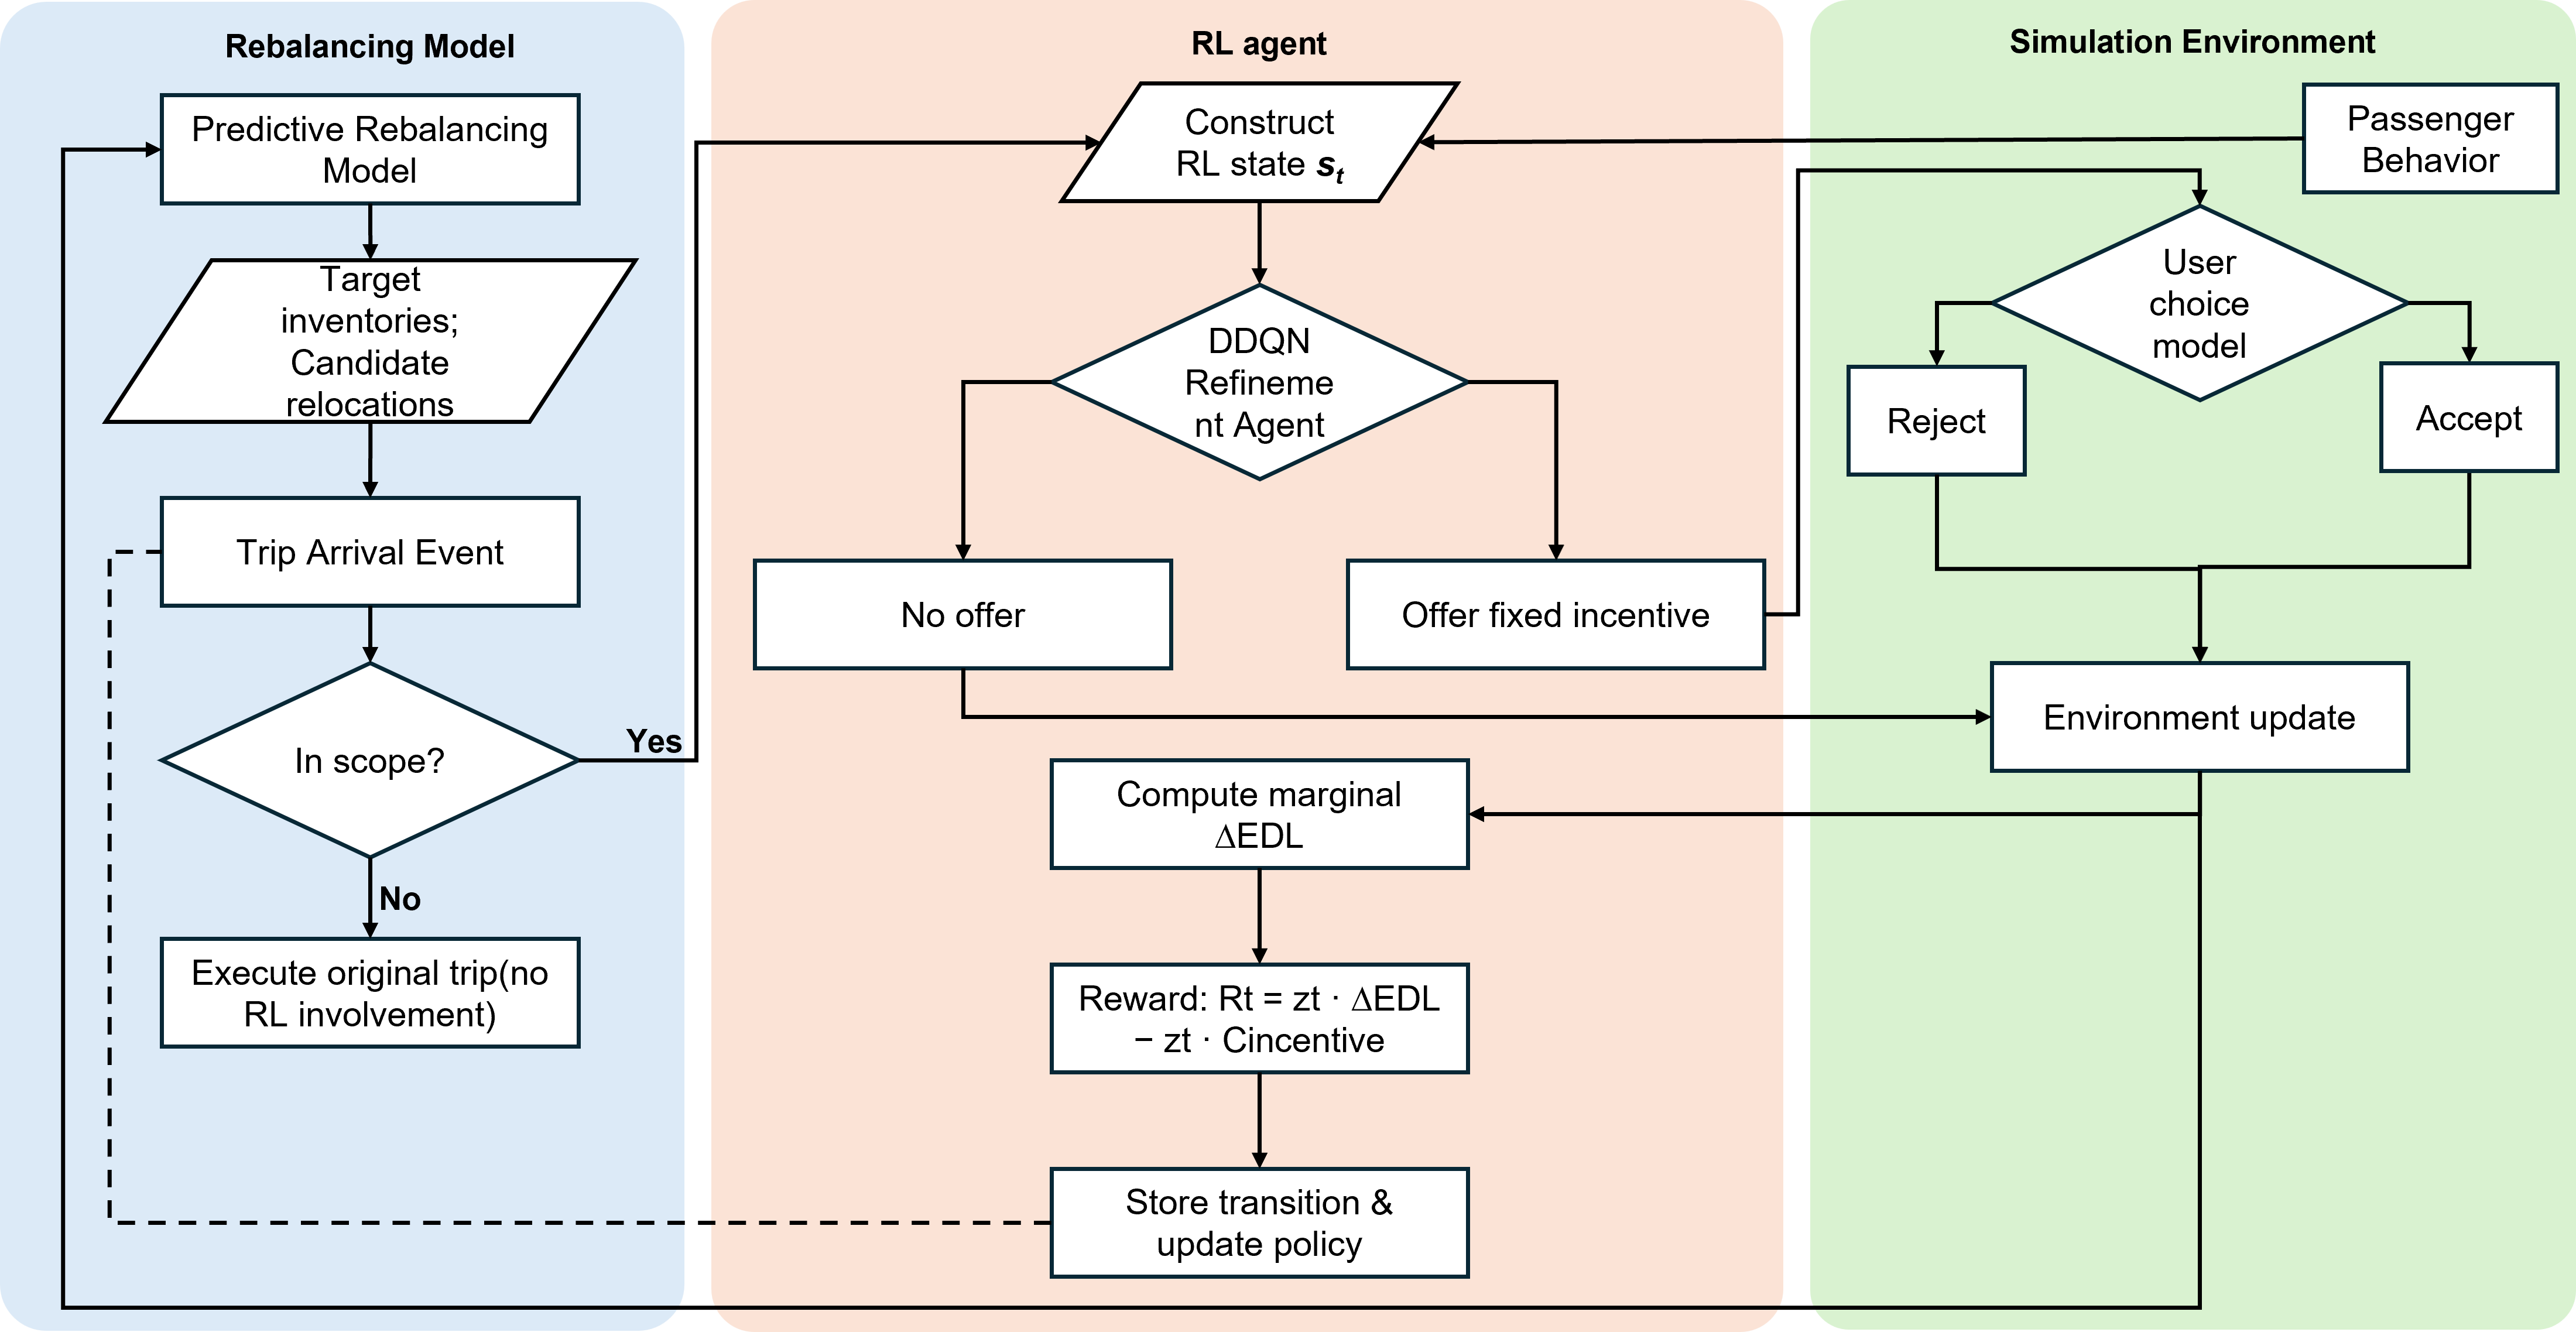
\includegraphics[width=1\textwidth]{figures/agent_structure.png}
    \caption{Event-driven execution workflow linking the upstream rebalancing model, the RL-based refinement agent, and the simulation environment.}
    \label{fig:methodology-workflow}
\end{figure}

The workflow is organized around trip events. A simulation episode begins with a pre-generated stream of trip requests, which are then processed in order of request time. For each arrival, the simulator first queries the external OR interface using the request origin, intended destination, and planning time slot. This determines whether the trip is associated with an eligible relocation opportunity from the upstream rebalancing model.

If no matching relocation opportunity exists, the request proceeds without RL involvement. If a match exists, the simulator does not immediately call the refinement layer. It first checks whether a rentable scooter is available at the origin zone. Requests for which no scooter is available are recorded as supply-related service loss and leave the decision process at that point.

Only requests that satisfy both conditions, namely OR matching and scooter availability, enter the refinement layer. The system state is then assembled from the observed operational context, including temporal, spatial, inventory, and offer-related information. The refinement policy chooses between two actions: do not activate the relocation offer, or activate the fixed incentive associated with the OR recommendation.

After the RL action is determined, the simulator evaluates a single-layer user choice. When no relocation offer is activated, the feasible user actions are to proceed with the original trip or to opt out. When the relocation offer is activated, the feasible user actions are to accept the offered relocation, keep the original destination, or opt out. The final behavioral outcome is thus one of three realized actions: offer, base, or opt\_out.

If the realized choice is offer, the effective destination becomes the recommended destination from the OR input. If the realized choice is base, the trip keeps its original destination. If the realized choice is opt\_out, the request leaves the execution process without being served. Otherwise, the trip is completed through scooter assignment, trip execution, battery-state transition, and an inventory update at the realized destination.


After the trip outcome is known, the simulator records the operational consequences of the decision. These include whether the trip was served, whether a relocation was accepted, and how the local state changed after execution. For RL-enabled runs, the simulator also stores the decision as a temporary transition and completes the reward calculation when the next relevant decision state is observed, or at the end of the episode. This delayed-reward design allows the framework to capture not only the immediate trip outcome, but also realized loss and downstream EDL-related effects that appear between consecutive decision points.

This workflow clarifies the methodological role of the refinement layer. The RL agent does not manage all trips, assign scooters, or generate new relocation targets. Its role is narrower: it decides whether an already available relocation opportunity from the upstream OR model should be implemented for an eligible trip request under the current system state.


\section{Simulation Environment}

The experimental setting is an event-driven simulator for a free-floating shared e-scooter system. The simulator represents the service area as a finite set of geo-fenced zones, tracks zone-level inventory by battery category, processes trip requests in event time, and updates the system state after each served trip. This environment provides the controlled setting in which OR-only execution and OR-plus-RL refinement can be compared.

\subsection{Spatial Representation and Capacity}

The service area is represented as a set of discretized service zones \parencite{momen2025}. Each zone can act as an origin or destination of a trip and is associated with a finite capacity. The primary spatial setup is built from a station-map representation, where zone identifiers are mapped to coordinates and adjacency is derived from walking-distance thresholds. A synthetic grid constructor remains available as a fallback or prototype mode, but it is not the main description of the thesis environment.

At the state level, each zone is represented by a compact inventory tuple: inactive scooters, low-battery scooters, and high-battery scooters. Low- and high-battery scooters are treated as rentable, while inactive scooters are physically present but not serviceable. This distinction is necessary because service availability depends on battery-aware inventory rather than on total fleet count alone. Capacity is also used in the EDL-related state and reward logic, where full and empty states affect expected future service loss.

% \subsection{Demand and Trip Generation}

% Demand enters the simulator through trip requests. Each request contains an origin zone, an intended destination zone, a request time, a trip duration, a trip distance, and a user type. The simulation engine generates requests for an episode in advance and then processes them in time order, preserving event-time dynamics within each planning interval.

% The default demand source for OR/RL experiments is OD-slot sampling based on expected flows. In this mode, expected demand is specified for origin-destination-time combinations and then sampled stochastically during the simulation. Alternative demand sources, including simpler Poisson generation, also remain available. For the RL workflow studied here, OD-slot sampling is especially useful because it allows demand density to be shaped around OR-matched opportunities while keeping the evaluation profile fixed.

\subsection{Trip Generation under Demand Uncertainty}

To simulate passenger arrivals at trip level while preserving consistency with the upstream OR layer, we generate requests from the aggregated OD expectation table and inject stochasticity only in the simulator.  
The OR model itself remains unchanged and still optimizes on aggregated demand inputs.

\paragraph{Mean demand construction.}
Let $\omega_{odt}$ denote the expected number of trips from origin zone $o$ to destination zone $d$ in time slot $t$, derived from the aggregated demand table (\texttt{omega\_h}).  
In the simulator, the slot-level mean is
\begin{equation}
\mu_{odt} = \omega_{odt} \cdot s_g \cdot s_w(t) \cdot s_{od}(o,d,t),
\end{equation}
where $s_g$ is a global scaling factor, $s_w(t)$ is an optional window-specific factor, and $s_{od}(o,d,t)$ is an optional OD-target factor (used for controlled stress/signal settings).

\paragraph{Arrival count distribution.}
A pure Poisson assumption is used as baseline, but the final setting adopts a Negative Binomial (NB2) arrival model to capture over-dispersion observed across days and time periods:
\begin{equation}
N_{odt} \sim \mathrm{NB2}(\mu_{odt}, \phi_t),
\end{equation}
with
\begin{equation}
\mathbb{E}[N_{odt}] = \mu_{odt}, \qquad
\mathrm{Var}(N_{odt}) = \mu_{odt} + \phi_t \mu_{odt}^2.
\end{equation}
Thus, $\phi_t=0$ reduces to the Poisson case, while $\phi_t>0$ increases variance without changing the mean.

\paragraph{Sampling implementation.}
NB2 is implemented via a Gamma--Poisson mixture:
\begin{equation}
\tilde{\lambda}_{odt} \sim \Gamma(k_t,\theta_{odt}), \quad
N_{odt} \sim \mathrm{Poisson}(\tilde{\lambda}_{odt}),
\end{equation}
with
\begin{equation}
k_t=\frac{1}{\phi_t}, \qquad \theta_{odt}=\frac{\mu_{odt}}{k_t},
\end{equation}
which guarantees the NB2 mean--variance structure above.

\paragraph{Dispersion profile calibration.}
Because only aggregated OD averages are available (instead of full day-level OD count sequences), we use a robust proxy calibration for $\phi_t$ by hour:
\begin{enumerate}
\item Compute network-level hourly totals $T(d,h)$ across day-of-week $d$.
\item For each hour $h$, compute coefficient of variation $\mathrm{CV}_h$ over $d$.
\item Map to dispersion using
\begin{equation}
\phi_h = \mathrm{clip}(a\cdot \mathrm{CV}_h + b,\ \phi_{\min},\ \phi_{\max}),
\end{equation}
with default $a=2.0$, $b=0.1$, $\phi_{\min}=0.05$, $\phi_{\max}=5.0$.
\end{enumerate}
The resulting profile is stored as \texttt{nb\_phi\_profile.csv} and loaded at runtime (\texttt{by\_hour} mode).  
This design is configurable and can be replaced by MLE-based estimation once day-level OD counts become available.

\paragraph{Trip-level event generation.}
For each sampled count $N_{odt}$, the simulator creates $N_{odt}$ trip requests by uniformly sampling a request time within slot $t$, fixing the origin and destination to $(o,d)$, drawing trip duration and distance from the existing simulator distributions, and sampling user type from the configured user-type prior.

\paragraph{Rationale.}
This design preserves OR--simulation consistency at the mean level (same aggregated demand source) while providing realistic stochastic variability for RL training and evaluation.  
In summary, OR remains an expectation-level optimizer, and the simulator emulates realized trip uncertainty around that expectation.


\subsection{Fleet and Battery-State Dynamics}

Fleet dynamics are tracked at the scooter level and aggregated to zone-level state variables. When a trip is served, the simulator selects an available scooter from the origin zone, removes it from the origin inventory, applies a trip completion event, updates its battery category, and adds it to the realized destination inventory. Scooter assignment follows scenario-specific rules that are discussed later in the thesis.

Battery evolution is modeled through a Markov transition mechanism over the inactive, low, and high categories \parencite{momen2025}. This allows the simulator to capture the operational fact that a scooter can remain physically present while becoming unavailable for future users. The resulting state transition is therefore not only spatial but also energy-dependent.

\subsection{User Response Modeling}

User behavior is part of the simulation environment rather than part of the RL policy. It is modeled as a single-layer discrete choice process aligned with the choice-model formulation used in the referenced e-scooter studies \parencite{burghardt2025behavioral,momen2025}. When no relocation offer is activated, the user chooses between proceeding with the original trip and opting out. When a relocation offer is activated, the user chooses among accepting the offered relocation, keeping the original destination, and opting out.

For an eligible decision event \(i\), define common user/context attributes
\[
\mathbf{z}_i=
\left[
\text{type}_{25},
\text{prev\_use},
\text{bike},
\text{income\_low},
\text{living\_alone},
\text{living\_shared},
\text{attitude},
\text{range\_anxiety}
\right]_i .
\]
The base and offer utilities are written as
\begin{equation}
\begin{aligned}
V_i^{(\textit{base})}
=\;&
\frac{1}{2}\beta_{ES}
+\beta_{walk}\,walk_i^{base}
+\beta_{unlock}\cdot 1
+\beta_{ride}\,c_i^{base}
+\beta_{batt}\,r_i^{base}
\\
&+
\beta_{type}\,\text{type}_{25,i}
+\beta_{prev}\,\text{prev\_use}_i
+\beta_{bike}\,\text{bike}_i
+\beta_{inc}\,\text{income\_low}_i
\\
&+
\beta_{alone}\,\text{living\_alone}_i
+\beta_{shared}\,\text{living\_shared}_i
+\eta_{att}\,\text{attitude}_i
+\eta_{range}\,\text{range\_anxiety}_i,
\end{aligned}
\end{equation}
\begin{equation}
\begin{aligned}
V_i^{(\textit{offer})}
=\;&
\frac{1}{2}\beta_{ES}
+\beta_{walk}\,walk_i^{offer}
+\beta_{unlock}\cdot 1
+\beta_{ride}\,c_i^{offer}
+\beta_{batt}\,r_i^{offer}
\\
&+
\beta_{type}\,\text{type}_{25,i}
+\beta_{prev}\,\text{prev\_use}_i
+\beta_{bike}\,\text{bike}_i
+\beta_{inc}\,\text{income\_low}_i
\\
&+
\beta_{alone}\,\text{living\_alone}_i
+\beta_{shared}\,\text{living\_shared}_i
+\eta_{att}\,\text{attitude}_i
+\eta_{range}\,\text{range\_anxiety}_i.
\end{aligned}
\end{equation}
The opt-out alternative is the reference utility:
\[
V_i^{(\textit{opt-out})}=0.
\]
The monetary/range sub-terms are
\[
c_i^{base}=p_{ride}\cdot rt_i^{base},
\qquad
c_i^{offer}=p_{ride}\cdot rt_i^{offer}-inc_i,
\]
\[
r_i^{base}=k_{range}\cdot batt_i^{base},
\qquad
r_i^{offer}=k_{range}\cdot batt_i^{offer}.
\]
When no offer is activated, the feasible set is \(\mathcal{A}_i=\{\textit{base},\textit{opt-out}\}\); when an offer is activated, \(\mathcal{A}_i=\{\textit{offer},\textit{base},\textit{opt-out}\}\).

Choice probabilities are computed with a softmax form over the feasible set \(\mathcal{A}_i\):
\[
P_i(a)=\frac{\exp\!\left(V_i^{(a)}\right)}{\sum_{b\in \mathcal{A}_i}\exp\!\left(V_i^{(b)}\right)}, \quad a\in\mathcal{A}_i.
\]
Accordingly, \(\mathcal{A}_i=\{\textit{base},\textit{opt-out}\}\) when no offer is activated, and \(\mathcal{A}_i=\{\textit{offer},\textit{base},\textit{opt-out}\}\) when an offer is activated. The realized user action is then sampled from \(P_i(\cdot)\).

\paragraph{Parameter interpretation.}
The utility parameters are grouped by behavioral meaning.  
\(\beta_{walk}\), \(\beta_{ride}\), and \(\beta_{unlock}\) capture sensitivity to access time and monetary trip cost components; \(\beta_{batt}\) captures the effect of battery-related range utility.  
\(\beta_{type}\), \(\beta_{prev}\), \(\beta_{bike}\), \(\beta_{inc}\), \(\beta_{alone}\), and \(\beta_{shared}\) represent user-attribute and context effects, while \(\eta_{att}\) and \(\eta_{range}\) capture latent attitude and range-anxiety effects.  
The constants \(p_{ride}\) and \(k_{range}\) define the price and range conversion terms used to map trip and battery attributes into utility inputs.  
In this chapter, these terms are defined at model level; the concrete coefficient values and default attribute settings used in experiments are reported in Chapter~7 (Table~\ref{tab:user-model-params}).

Accordingly, the RL policy does not determine the final user choice. It decides only whether the relocation offer is activated, after which the realized user action is sampled from the corresponding choice set.

\section{OR Interface and Refinement Boundary}

\subsection{External OR Interface}

The upstream rebalancing model enters the simulator through an external OR interface. As a result, the simulator does not depend on the internal optimization structure of the upstream model. It consumes only execution-relevant outputs that have already been translated into a standardized relocation table, denoted as \texttt{U\_odit}.

Each row of \texttt{U\_odit} defines one candidate relocation opportunity. The table specifies the origin zone, the original destination zone, the recommended destination zone, the planning time slot, the incentive amount, and the associated relocation quota. At runtime, the simulator queries this table using the realized request origin, intended destination, and request-time slot. If a matching opportunity with remaining quota exists, the request is treated as eligible for refinement-layer intervention. Otherwise, it proceeds outside the OR-guided relocation context.

This interface makes the refinement problem modular. The simulator can evaluate trip-level execution decisions without depending on how the upstream OR model was formulated, calibrated, or solved. The thesis therefore studies the execution consequences of OR-generated guidance rather than the internal mechanics of OR plan generation.

\subsection{Refinement Boundary}

The role of the refinement layer is deliberately narrow. It does not generate relocation intent independently, does not compute new target inventories, and does not re-optimize the upstream plan. Instead, it operates only on relocation opportunities that already exist in the OR input and decides whether a matched opportunity should be activated for a realized trip request.

This boundary is important for the thesis contribution. The proposed policy is not a full rebalancing controller. It does not choose among arbitrary destinations or redesign the global allocation of vehicles across the network. The recommended destination is already fixed by the OR input when the refinement decision is made. The RL policy therefore acts on only one operational degree of freedom: whether to activate or suppress an already available relocation offer.

The same logic applies to quota handling. Quota is defined by the OR input and managed by the OR interface according to the selected quota-consumption rule. The refinement layer does not modify quota values or create additional relocation opportunities. It only interacts with the currently available opportunity and its remaining execution feasibility.

Defining the refinement boundary in this way keeps the research problem well posed. It ensures that the thesis remains focused on selective execution of interval-based relocation guidance rather than drifting into joint planning-and-control optimization. It also makes the later evaluation easier to interpret: any observed difference between OR-only execution and OR-plus-RL execution can be attributed to trip-level activation decisions rather than to changes in the upstream relocation plan itself.


\section{Trip-Level Refinement Problem}

\subsection{Decision Epoch}

The refinement layer faces a binary decision at eligible OR-matched trip events. A decision epoch occurs only when the simulator has identified a relocation opportunity for the arriving request and a rentable scooter is available at the origin zone. This definition is narrower than all trip arrivals and reflects the actual operational role of the refinement layer.

At each such decision epoch, the policy receives a state representation constructed from the current system context. The resulting action is then interpreted as an execution decision: suppress the relocation offer or activate the fixed incentive offer associated with the OR recommendation.

\subsection{State Representation}

The state representation is designed to capture the local execution context of an OR-matched trip event in a compact but operationally meaningful form. Rather than describing the entire network in full detail, the state focuses on the information that is most directly relevant for deciding whether an available relocation opportunity should be activated under the current system conditions.

The state combines five groups of information. First, it includes a temporal feature that indicates the current position of the request within the episode. Second, it contains spatial identity features for the origin, the original destination, and the recommended destination associated with the matched OR opportunity. Third, it includes battery-aware inventory features for these same three zones. Fourth, it contains EDL-related features that summarize the local expected-loss context at the decision time. Fifth, it includes trip-level and offer-level attributes that characterize the immediate operational trade-off of activating the relocation option.

To avoid notation conflict with decision-step indexing, this thesis uses \(R_i\) for the recommended destination zone associated with decision step \(i\), while \(i\) itself always denotes the decision-step index.

Table~\ref{tab:state-features} summarizes the variables included in the current state vector.

\begin{table}[H]
\centering
\caption{State variables used in the current trip-level refinement policy.}
\label{tab:state-features}
\begin{tabular}{p{3.2cm}p{5.4cm}p{5.2cm}}
\toprule
\textbf{Feature group} & \textbf{Variables} & \textbf{Meaning} \\
\midrule
Temporal context
& \texttt{slot\_norm}
& Normalized position of the current request within the episode, derived from the planning slot. \\

Spatial identity
& \texttt{origin\_id}, \texttt{destination\_id}, \texttt{recommended\_id}
& Normalized identifiers of the origin zone, original destination zone, and recommended destination zone. \\

Origin-zone inventory
& \texttt{o\_n}, \texttt{o\_l}, \texttt{o\_h}
& Normalized inactive, low-battery, and high-battery scooter counts at the origin zone. \\

Original-destination inventory
& \texttt{d\_n}, \texttt{d\_l}, \texttt{d\_h}
& Normalized inactive, low-battery, and high-battery scooter counts at the original destination zone. \\

Recommended-destination inventory
& \texttt{r\_n}, \texttt{r\_l}, \texttt{r\_h}
& Normalized inactive, low-battery, and high-battery scooter counts at the recommended destination zone. \\

EDL context
& \texttt{edl\_o}, \texttt{edl\_d}, \texttt{edl\_r}
& EDL-related features for the origin, original destination, and recommended destination at the decision time. \\

Trip and offer attributes
& \texttt{rt\_base}, \texttt{rt\_offer}, \texttt{walk\_extra}, \texttt{incentive}
& Base ride time, ride time under relocation, additional walking time, and fixed incentive amount. \\

Resource context
& \texttt{quota\_remaining}, \texttt{budget\_remaining}
& Remaining quota of the matched relocation opportunity and remaining budget-related context passed to the decision layer. \\
\bottomrule
\end{tabular}
\end{table}


Taken together, the state representation is intentionally local, structured, and decision-oriented. It combines temporal position, spatial identity, battery-aware local inventory, EDL signals, and offer attributes into a single vector that is informative enough for trip-level selective execution while avoiding the complexity of a full-network end-to-end representation.



\subsection{Action Space}

The action space is binary. Action 0 suppresses the relocation offer, so the user faces the no-offer choice set and may either proceed with the original trip or opt out. Action 1 activates the fixed relocation incentive, so the user faces the offer-enabled choice set and may choose the relocation option, keep the original destination, or opt out.

This restricted action space is intentional. It keeps the refinement mechanism interpretable, avoids turning the thesis into a continuous pricing problem, and aligns the policy with the core operational question: whether an existing relocation suggestion should be activated for a realized trip request.


\subsection{Sources of Uncertainty}

The execution outcome remains uncertain even after the binary action is selected. User response is one source of uncertainty, because the realized behavioral outcome depends on the choice set induced by the RL action and may end in offer, base, or opt\_out. Future trip arrivals are stochastic under the OD-slot demand process. Battery transitions and subsequent inventory evolution also affect future service availability. As a result, the same relocation suggestion may have different operational value depending on the realized state when the trip arrives.

\section{RL Formulation and Policy Logic}

\subsection{Sequential Decision Perspective}

The refinement problem is formulated as a sequential decision problem. Each eligible decision produces a state, an action, a realized outcome, and a transition to a later decision state. This perspective is appropriate because an accepted relocation affects not only the current trip but also future inventory distribution, battery composition, and service availability at later decision times.

The learning setup uses a value-based binary policy. The RL agent is a Double Deep Q-Network (DDQN), which is well suited to the low-dimensional discrete action space and helps reduce the overestimation bias associated with standard DQN. The agent therefore serves as a selective execution policy rather than replacing the upstream OR model.

\subsection{Reward Design}

The reward evaluates trip-level execution decisions in terms of both their immediate operational consequences and their expected downstream effect on system performance. The aim is not to maximize the number of issued offers, but to activate relocation opportunities only when they are likely to improve service-related outcomes while avoiding unnecessary incentive expenditure.

One design choice is to compute reward in delayed form rather than assign it immediately at the moment of action selection. This is necessary because the operational effect of an execution decision is not fully observable at the instant when the offer is activated or suppressed. Some consequences emerge only after the trip outcome is realized and subsequent system evolution reveals whether service loss occurred before the next relevant decision point. The simulator therefore stores each RL decision as a pending transition and finalizes its reward when the next RL decision state becomes available, typically at the next offer opportunity, or at the end of the episode.

The reward combines five components: a realized-loss term, an EDL-improvement term, an acceptance incentive term, a realized-cost term, and a rejection penalty. In compact form, the reward is defined as
\begin{equation}
    r_i
    =
    - w_L \widetilde{L}_i
    +
    w_E \widetilde{\Delta EDL}_i
    +
    \beta_a Acc_i
    -
    \beta_c Cost_i
    -
    \beta_r Rej_i.
\end{equation}

Here, \(L_i\) is the realized no-supply loss over the decision window from decision step \(i\) to the next decision step (or episode end), restricted to the three involved zones \(O_i\), \(D1_i\), and \(R_i\). \(\Delta EDL_i\) is the expected-demand-loss difference induced by the realized action outcome under the fixed OR guidance. \(Acc_i\in\{0,1\}\) indicates whether the relocation option is realized, \(Cost_i\) is realized incentive payout (counted only when relocation is realized), and \(Rej_i\in\{0,1\}\) indicates activated-but-not-accepted outcomes. The coefficients \(w_L,w_E,\beta_a,\beta_c,\beta_r\) control the relative contribution of these components.

To stabilize training signals across episodes, the realized-loss and EDL-improvement components are normalized and clipped as
\begin{equation}
\widetilde{L}_i
=
\mathrm{clip}\!\left(
\frac{L_i}{L_{ref}},\,0,\,1
\right),
\end{equation}
\begin{equation}
\widetilde{\Delta EDL}_i
=
\mathrm{clip}\!\left(
\frac{\Delta EDL_i}{E_{ref}},\,-1,\,1
\right),
\end{equation}
where \(L_{ref}>0\) and \(E_{ref}>0\) are scaling constants, and
\[
\mathrm{clip}(x,a,b)=\min\{\max(x,a),\,b\}.
\]

The first component, \(L_i\), captures realized short-horizon service loss between two consecutive refinement decisions. Let \(\tau_i\) denote the event time of decision step \(i\). Then \(L_i\) is counted over the event window \((\tau_i,\tau_{i+1}]\), or until episode end if no subsequent decision occurs. The counting scope is restricted to the three zones involved in the current decision context: origin \(O_i\), original destination \(D_i\), and recommended destination \(R_i\). This term counts realized no-supply loss events (rather than user opt-out events), and therefore reflects operational deterioration in available service capacity.

The second component, \(\Delta EDL_i\), captures the change in expected demand loss induced by the realized action outcome. This term compares cumulative EDL under a baseline no-relocation counterfactual with cumulative EDL under the realized post-decision state over the fixed look-ahead horizon (2 hours). A positive value indicates that the realized execution outcome is expected to reduce future demand loss relative to not activating relocation.

The normalization anchors \(L_{ref}\) and \(E_{ref}\) are numerical scaling references for comparability and stability, not physical constants. In implementation, both are calibrated from decision-level samples collected across many episodes and seeds using high quantiles (current setup: P95). Specifically, \(L_{ref}\) is estimated from the sample distribution of \(L_i\), and \(E_{ref}\) from \(|\Delta EDL_i|\), with lower-bound guards to avoid degenerate scaling in sparse regimes.

The third component, \(Acc_i\), rewards behaviorally effective activations when the user chooses the offered relocation option (\(Acc_i=1\) if accepted, otherwise \(0\)). The fourth component, \(Cost_i\), represents realized incentive expenditure. Incentive cost is counted only when the relocation option is actually chosen, rather than whenever an offer is only activated. This choice reflects the operational fact that financial payout is incurred only when the user accepts the offered relocation.

The fifth component, \(Rej_i\), penalizes activated offers that do not result in the relocation option being chosen (\(Rej_i=1\) for activated-but-not-accepted offers, otherwise \(0\)). This includes cases where the offer is activated but the realized user choice is not \textit{offer} (i.e., \textit{base} or \textit{opt-out}). This term discourages the policy from activating relocation offers that are unlikely to be behaviorally effective.

Taken together, the reward design reflects the core logic of the refinement layer. The policy should prefer decisions that reduce short-term realized loss, improve future expected demand-loss conditions, activate behaviorally effective offers, avoid unnecessary incentive payout, and refrain from activating offers that are unlikely to be effective. In the current baseline setup, \(w_L=w_E=0.5\), while \(\beta_a\), \(\beta_c\), and \(\beta_r\) are tuned through sensitivity analysis.


\subsection{Training and Evaluation Interface}

The training and evaluation interface assesses the refinement layer as an execution policy operating on top of externally provided rebalancing guidance. In this framework, the upstream OR input remains fixed, while the trip-level policy is trained and evaluated through repeated simulation episodes. This makes it possible to isolate the value of selective execution without conflating it with changes in the planning layer.

From a learning perspective, each episode consists of a sequence of realized trip events processed in event time. Whenever an eligible relocation opportunity arises, the current system state is translated into a policy input, an execution action is selected, and the resulting transition is recorded for learning or evaluation. The simulator thus provides the interaction environment, while the refinement policy is the only component that changes across training and policy-comparison runs.

The training interface is therefore based on repeated environment rollouts under controlled demand and OR-input conditions. During training, the policy explores the action space through stochastic action selection, while observed transitions are stored and used to update the value function. During evaluation, the learned policy is executed without exploratory noise so that its decision behavior can be compared consistently against non-learning baselines. This distinction matters because the objective of the thesis is not only to learn a policy, but also to assess whether the learned execution rule improves operational outcomes relative to simpler alternatives.

Eligible relocation opportunities may be sparse under the target demand distribution. The broader training interface therefore allows different demand-density settings for policy development and final assessment. In particular, a denser demand configuration can be used to expose the policy to more matched relocation opportunities during training, while the final evaluation remains fixed on the target distribution of interest. This does not change the decision problem itself; it addresses the practical issue that sparse decision opportunities can weaken the learning signal if the policy is trained only under the final evaluation distribution.

The evaluation interface compares policies under identical simulation conditions, including the same OR input structure, the same demand-profile specification, and controlled seed schedules. This ensures that differences in observed performance can be attributed to the execution policy rather than to changes in the upstream guidance or the simulation configuration. The main evaluation outputs are therefore interpreted as comparative execution outcomes, not as evidence that the OR plan itself has improved.

Overall, the training and evaluation interface has two purposes: it provides a reproducible procedure for fitting a trip-level execution policy within the proposed framework, and it establishes a fair comparison setting in which OR-only execution and OR-guided refinement policies can be assessed on the same operational basis.


\section{Reproducibility and Configuration Logic}

The methodology is organized in a configurable simulation workspace. Random seeds, planning intervals, episode horizons, OR input paths, demand-source settings, omega sampling profile parameters, reward coefficients, and RL hyperparameters are specified explicitly through configuration files or command-line overrides. This structure allows the same core simulator to be used for OR-only baselines, single-stage RL training, and multi-profile evaluation.

The default OR/RL demand path uses OD-slot expected flows with profile scaling during the simulation. Replay-based demand remains available, but it is not the default for the RL protocol used in this thesis. This distinction is important for reproducibility because the experimental protocol must specify not only the simulator but also the demand distribution under which the policy is trained and evaluated.

The simulator also records transition-level information for RL analysis, including state, action, next state, reward, accepted flag, rejected flag, EDL change, realized loss, and cost term. These logs support later experimental comparison and help diagnose whether the refinement layer is learning from a sufficient number of decision opportunities.

\section{Chapter Summary}

This chapter has presented the methodology as an event-driven execution framework that connects external OR guidance, a battery-aware e-scooter simulation environment, a single-layer user choice model, and a DDQN-based binary refinement policy. The key methodological boundary is that the RL agent does not generate relocation plans or alternative destinations. Instead, it decides only whether an already available OR relocation opportunity should be activated at an eligible trip event.

The chapter also formalized the simulator-side decision logic: only OR-matched requests with available rentable scooters enter the refinement decision point; user behavior is then realized through one-step choice among feasible actions (\textit{offer/base/opt-out}); and system dynamics are updated through trip execution, battery transition, and zone inventory updates.

For learning, the refinement layer is formulated as a sequential decision process with delayed transition finalization and a hybrid reward that combines realized service-loss feedback, EDL-improvement signal, realized incentive cost, and rejection penalty. Together, these design choices provide a reproducible and modular basis for comparing OR-only execution with OR+RL selective execution in the next chapter.
